
\documentclass[12pt, a4paper]{article}

\usepackage[utf8]{inputenc}
\usepackage[T1]{fontenc}
\usepackage[russian]{babel}
\usepackage[oglav,spisok,boldsect,eqwhole,figwhole,hyperref,hyperprint,remarks,greekit]{./style/fn2kursstyle}
\graphicspath{{./style/}{./figures/}}

\usepackage{multirow}
\usepackage{supertabular}
\usepackage{multicol}
% Параметры титульного листа
\title{Нахождения уравнения\\ изгиба балки}
\author{В.\,Г.~Пиневич}
\supervisor{А.\,В.~Чередниченко}
\group{ФН2-41Б}
\date{2022}

% Переопределение команды \vec, чтобы векторы печатались полужирным курсивом
\renewcommand{\vec}[1]{\text{\mathversion{bold}${#1}$}}%{\bi{#1}}
\newcommand\thh[1]{\text{\mathversion{bold}${#1}$}}
%Переопределение команды нумерации перечней: точки заменяются на скобки
\renewcommand{\labelenumi}{\theenumi)}
\begin{document}

\maketitle

\tableofcontents



\newpage

\section-{Введение}
Проблема вычисления уравнение прогиба балки возникает во многих задачах, в частности в строительной механике. В силу наличия большого числа действующих сил и моментов решение такой задачи классическим методом, т.е. вычислением дифференциального уравнения вызывает сложности в виду большого числа граничных условий. Однако с развитием теории обобщенных функций и сопротивление материалов было найдено более удобный способ расчета прогиба балки. Данная работа посвящена анализу методов решения подобных задач, выделение их недостатков и преимуществ.

\section{Постановка задачи}
Для расчета уравнения гибкого стержня необходимо ввести несколько понятий. $q$~---~распределенная нагрузка, $Q$~---~сосредоточенная сила, $M$~---~момент.

\subsection{Чистый изгиб}
Обратимся к источнику~\cite{Feofociev}.
Рассмотрим стержень, закрепленный произвольным образом. Выделим часть стержня длинно $dz$ и приложим поперечные силы $Q + dQ$ и моменты $M + dM$. Поскольку $dz$ мало, то можно считать нагрузку равно распределенной~(рис. \ref{pic1}).
\begin{figure}[!h]
	\centering
	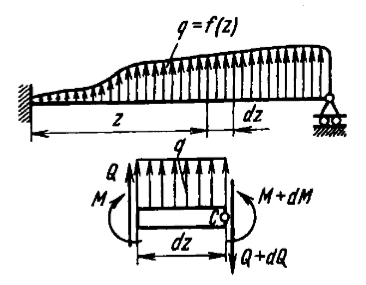
\includegraphics[width=0.35\textwidth]{pic.1}%
	\caption{Равно распределенная нагрузка}
	\vspace*{-2mm}
	\label{pic1}
\end{figure}
\\Имеем состояния равновесия:  
\begin{equation}
	\label{systemB}
	\begin{cases}
	\sum\limits {{F_z = 0}} \\
	\sum\limits {{M_z = 0}}
	\end{cases}
	\Leftrightarrow
	\begin{cases}
		Q + q dz - Q - Q dz = 0 \\
		M + Q dz + q dz \frac {dz}{z} - M -dM = 0
	\end{cases}
\end{equation}
Выражение $q dz \frac {dz}{z}$ можно отбросить,
как величину высшего порядка малости.

Из системы~(\ref{systemB}) следует, что если балка нагружен только сосредоточенными силами, то $q = 0$, $Q = const$, $M$~---~линейная функция от $z$, если $q = const$, то функция $Q$ будет линейной.

Итого из системы~(\ref{systemB}) получаем:
\begin{equation}
	\label{QM}
 \frac {dQ}{dz} = q, 
 \frac {dM}{dz} = Q,
\end{equation}

Далее рассмотрим наиболее простой случай изгиба~---~чистый изгиб. Под таким видом изгиба понимаются случаи, при которых в поперечных сечениях стержня возникают только изгибающие моменты, а $Q = 0$. Для участок балки, где это условия выполнятся $M = const$~\eqref{QM}. Рассмотрим только этот участок. На нем стержень изогнется по действием моментов $M$. Тогда при условии, что сечение балки однородное, в любом сечении будет одинаковй момент, а значит изменение кривизны стержня будет одинаковым. Следовательно, при чистом изгибе ось однородной балки принимает форму дуги окружности.

Разрезая стержень на равные части сечением \emph{А--А}, получаем участки вдвое меньше~(рис. \ref{pic2}), которое все еще остается плоским в силу того, что обе стороны являются полностью равноценными. Процесс деления можно проложить дальше. Таким образом доказано, что в неограниченной области близости от любого заданного сечения можно задать бесконечно много сечений, которые в совокупности будут эквивалентны искомому. Это утверждение является точным для чистых сечений, для остальных видов является приближенным.
\begin{figure}[!h]
	\centering
	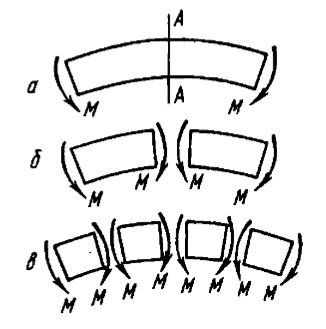
\includegraphics[width=0.5\textwidth]{pic.2}%
	\caption{Сечение \emph{А--А}}
	\vspace*{-2mm}
	\label{pic2}
\end{figure}

\newpage Деформацию можно рассматривать как поворот плоских поперечных сечений относительно друг друга~(рис. \ref{pic3}).
\begin{figure}[!h]
	\centering
	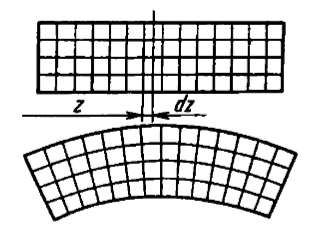
\includegraphics[width=0.35\textwidth]{pic.3}%
	\caption{Деформация плоского поперечного сечения}
	\vspace*{-2mm}
	\label{pic3}
\end{figure}
\\ Рассмотрим два смежных сечения, расположенных на растоянии $dz$~(рис. \ref{pic4}). Примем левое сечение за неподвижное. При повороте правого сечения на угол $d\theta$ верхние слои удлинятся, нижние -- укоротятся. Слой, который не изменится назовем нейтральным и обозначим \emph{CD}. После поворота кривизна нейтрального слоя изменится следующим образом: 
\begin{equation}
	\label{1/qq}
	\frac {1}{\rho} = \frac {d\theta}{dz}, 
\end{equation}
Случайный отрезок $AB = dz$ ~(рис. \ref{pic4}) получит приращение $A'B' - AB$. С учетом того, что сечение остается плоским, $A'B' - AB = (\rho + y)d\theta - \rho d\theta = yd\theta$, где $y$ --- расстояние от $AB$ до $CD$. 
\begin{figure}[!h]
	\centering
	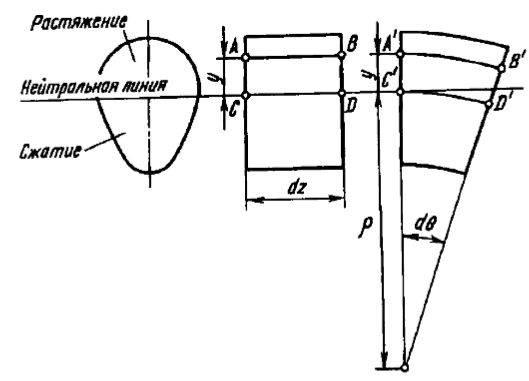
\includegraphics[width=0.5\textwidth]{pic.4}%
	\caption{Образование деформации при чистом изгибе}
	\vspace*{-2mm}
	\label{pic4}
\end{figure}

Относительное удлинение $AB$ равно 
\begin{equation}
	\label{eps}
	\varepsilon = \frac {y d\theta}{dz} = \frac{y}{\rho}.
\end{equation}

По закону Гука, 
\begin{equation}
	\label{guka}
	\sigma = E \varepsilon = E \frac{y}{\rho}.
\end{equation}
Геометрические место точек в сечении, где напряженность $\sigma = 0$, называется нейтральной линией сечения.
\begin{figure}[!h]
	\centering
	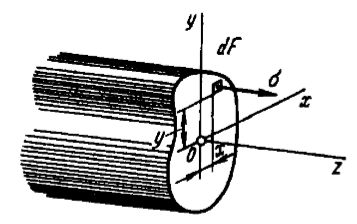
\includegraphics[width=0.35\textwidth]{pic.5}%
	\caption{Сечение балки}
	\vspace*{-2mm}
	\label{pic5}
\end{figure}

Сумма сил $\sigma d F$ ~(рис. \ref{pic5}) образует нормальную силу $N$ в сечении. При чистом изгибе $N = 0$, поэтому $N = \int_{F} \sigma d F = 0$, с учетом~\ref{guka}, $\frac{E}{\rho} \int_{F} y d F = 0$, откуда 
\begin{equation}
	\label{ydF}
	\int_{F} y d F = 0.
\end{equation}
Получили статический момент относительно нейтральной линии. Поскольку он равен нулю, нейтральная линий проходит через центр тяжести сечения. Таким образом мы можем определить координату $y$ в выражениях~(\ref{eps}), ~(\ref{guka}): она отсчитывается от центральной оси, перпендикулярной плоскости кривизны. Аналогично определяется и кривизна $\frac{1}{\rho}$, как кривизна оси стержня. 

Зададим систему координат $x, y, z$, связанную с сечением ~(рис. \ref{pic5}). Начало координат $O$ совместим с центром тяжести сечения. Ось $z$ направим по нормали к сечению, $x$ --- по нейтральной линии. Ось $y$ лежит в плоскости кривизны.

Изгибающий момент в поперечном сечении стержня, как и нормальная сила, может быть выражен через напряжения $\sigma$. 
\begin{equation}
	\label{bendM}
	\int_{F} \sigma x d F = M_y, \int_{F} \sigma y d F = M_x
\end{equation}

Стоит отметить, что изменение кривизны стержня происходит не обязательно в плоскости изгибающего момента.

При указанных условиях момент сил $\sigma d F$ относительно оси $y$ равен нулю, а относительно $x$ -- полному избегающему моменту $M$. Тогда получаем
\begin{equation}
	\label{bendM2}
	\frac{E}{\rho} \int_{F} y x d F = 0, \frac{E}{\rho} \int_{F} \sigma y^2 d F = M.
\end{equation}

Первое выражение сводится к $J_{xy} = 0$, т.е. изменение кривизны стержня происходит в плоскости момента в том случае, если последняя проходит через одну из главных осей сечения.

Из выражений ~(\ref{bendM2}) получаем зависимость кривизны стержня от изгибающего момента:
\begin{equation}
 	\label{rhoM}
 	\frac{1}{\rho} = \frac{M}{E J_{x}}, 
 \end{equation}
где $J_{x}$ --- момент инерции сечения относительно главной центральной оси, перпендикулярной плоскости изгибающего момента, $E$~---~модуль упругости, $M$ - изгибающий момент. Величина $E J_{x}$ называется жесткостью стержня при изгибе.

Для стержня круглого сечения с диаметром $D$:
\begin{equation}
	\label{Jround}
	J_{x} = \frac{\pi D^4}{64}.
\end{equation}

Для стержня прямоугольного сечения со сторонами $b, h$:
\begin{equation}
	\label{Jsq}
	J_{x} = \frac{b h^3}{12}.
\end{equation}

\subsection{Дифференциальное уравнение равновесия стержня}
Форму изогнутого стержня можно определить при помощи выражения ~(\ref{rhoM}). В неподвижной системе координат $yOz$~(рис. \ref{pic6}). 
\begin{equation}
	\label{diffbalkf}
	\frac{1}{\rho} = \frac{y''}{(1 + y'^2)^{\frac{3}{2}}}.
\end{equation}

Поскольку мы рассматриваем случай малых перемещений, то тангенс $ \theta$ между касательной к упругой линии изгиба и осью $z$ мал. Поэтому квадратом $y'$ можно пренебречь. и принять
\begin{equation}
	\label{diffbalkcurve}
	\frac{1}{\rho} \approx y'',
\end{equation}
\\откуда 
\begin{equation}
	\label{diffbalk}
	y'' = \frac{M}{E J_{x}}.
\end{equation}

Таким образом, мы получили дифференциальное уравнение стержня~(\ref{diffbalk}). 
Сопоставим выражения~(\ref{QM}) и~(\ref{diffbalk}), получаем четыре выражения, которые объясняют физический смысл производных 1--4 порядков соответственно:
\begin{equation}
	\label{diffbb4}
	\theta = y',~M = E J_{x} y'',~Q = E J_{x} y''',~
	q_{y} = E J_{x} y^{IV}.
\end{equation}
$y' = \theta$ --- угол поворота сечения, $y''$, $y'''$, $y^{IV}$ прямо пропорционально зависят от момента $M$, точечной силы $Q$, распределенной нагрузки $q$ соответственно. В свою очередь, $y$ --- отклонение точек осевой линии стержня от ее положения в недеформированном состоянии.

\begin{figure}[!h]
	\centering
	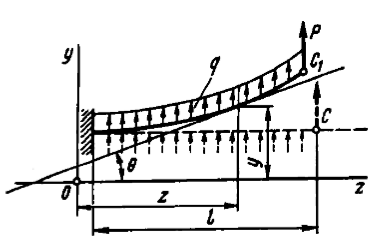
\includegraphics[width=0.35\textwidth]{pic.6}%
	\caption{Упругая линия изгиба балки}
	\vspace*{-2mm}
	\label{pic6}
\end{figure}
\newpage
Целью данной работы является изучение двух методов его решения: начальных коэффициентов и с помощью обобщенных функций. Будут рассмотрены два вида задач: балка в консольной заделке и двух опорный стержень. После решения этих задач будут сделаны выводы о эффективности и удобности рассмотренных методов.

\section{Теоретическая часть}

\subsection{Метод начальных коэффициентов}
Обратимся к источнику~\cite{Feofociev}.
Выражения~(\ref{diffbb4}) можно представить в виде системы дифференциальных уравнений первого порядка:
\begin{equation}
	\label{diffb4}
	\begin{cases}
		\frac{d Q}{d z} - q_{y}(z) = 0\\
		\frac {d M}{d z} - Q = 0\\
		\frac{d \theta}{d z} - \frac{M}{E J_{x}(z)} = 0\\
		\frac{d y}{d z} - \theta = 0, 
	\end{cases}
\end{equation}

В результате решения системы~(\ref{diffb4}) получаем отклонение точек осевой линии стержня от ее положения в недеформированном состоянии $y$, что и будет являться ответом.

\subsection{Метод обобщенных коэффициентов}
Обратимся к источнику~\cite{Korneev}.
В 1926 г. английский физик Дирак ввёл в квантовой механике символ $\delta (z)$, названный им дельта функцией.

Дельта функцию~(рис. \ref{dirac}) можно определить как 
\begin{equation}
	\label{diraca}
	\int_{-\infty}^z \delta (z - a) \varphi (z) dz = 
		\begin{cases}
			\infty, z < a \\
			0, z \geqslant a	
		\end{cases}
\end{equation}
\begin{figure}[!h]
	\centering
	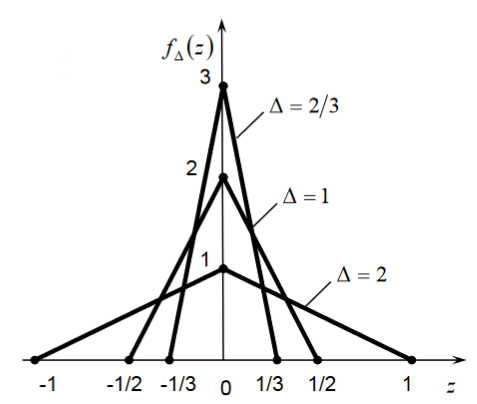
\includegraphics[width=0.35\textwidth]{dirac}%
	\caption{Возможное представление функции Дирака ~(\ref{diraca})}
	\vspace*{-2mm}
	\label{dirac}
\end{figure}

Функция Хевисайда определяется как
\begin{equation}
	\label{heavicase}
	H(z - a) = 
	\begin{cases}
		0, z < a \\
		1, z \geqslant a	
	\end{cases}
\end{equation}
Она обладает следующими свойствами:
\begin{equation}
	\label{heavicase}
	[H(z - a)]^\alpha = H(z - a),~
	H(z - a) H(z - b) = H(z - b),	
\end{equation}
т. е. при возведении в любую степень $0 > \alpha$ функция Хевисайда остаётся
неизменной, при перемножении двух функций Хевисайда результат равен
тому сомножителю, у которого сдвиг координаты больше: $a > b$.

\begin{figure}[!h]
	\centering
	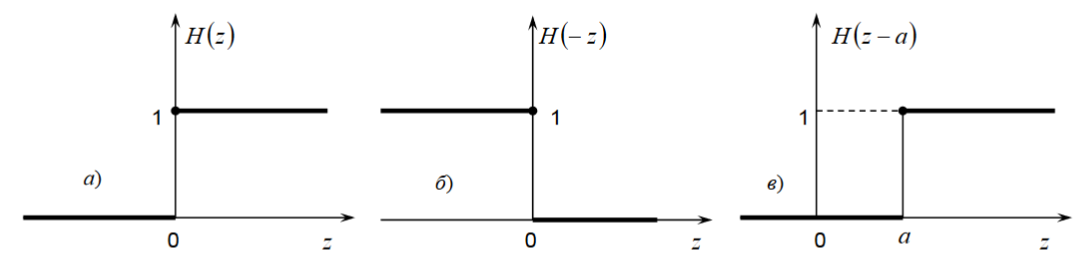
\includegraphics[width=0.75\textwidth]{heavi}%
	\caption{Единичная функция Хевисайда~(\ref{heavicase})}
	\vspace*{-2mm}
	\label{heavi}
\end{figure}

Если взять $\varphi (z) = 1$, получим соотношение, 
\begin{equation}
	\label{heavi}
	\int_{-\infty}^z \delta (z - a) dz = 
	H(z)
\end{equation}
которое связывает функцию Дирака и функцию Хевисайда~(рис. \ref{heavi}).

При решении задач сопротивления материалов достаточно располагать двумя табличными интегралами, содержащими обобщенные функции
Дирака и Хевисайда:
\begin{equation}
	\label{dirakint}
	\int_0^z f(z) \delta(z - a) d z = f(a)H(z - a),
\end{equation}
\begin{equation}
	\label{heaviint}
	\int_0^z f(z) H(z - a) d z = H(z - a)\int_a^z f(z) d z.
\end{equation}
\newpage
При интегрировании функции Хевисайда будем получать луч:
\begin{figure}[!h]
	\centering
	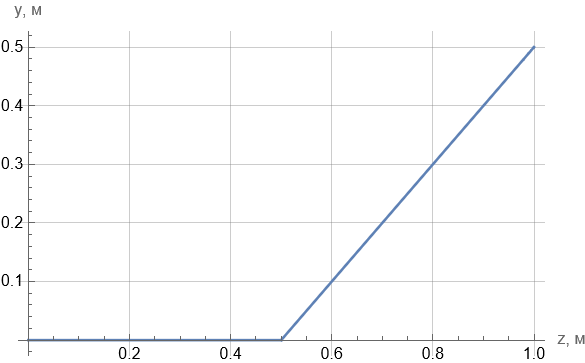
\includegraphics[width=0.45\textwidth]{intHeav}%
	\caption{Интеграл функции Хевисайда~(\ref{heavi})}
	\vspace*{-2mm}
	\label{intHeav}
\end{figure}
\newline
При повторном интегрировании функции Хевисайда будем получать полупараболу:
\begin{figure}[!h]
	\centering
	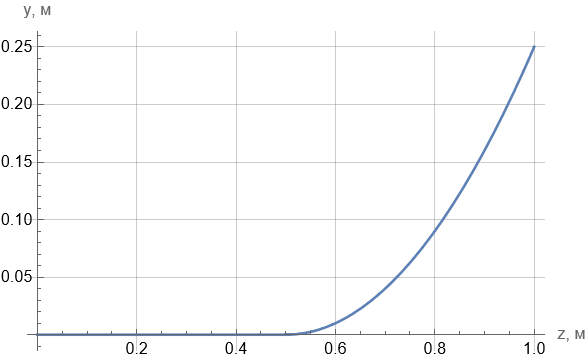
\includegraphics[width=0.45\textwidth]{int2Heav}%
	\caption{Повторный интеграл функции Хевисайда~(\ref{heavi})}
	\vspace*{-2mm}
	\label{int2Heav}
\end{figure}
\newline
Последний график~(рис. \ref{int2Heav}) по форме сильно напоминает изгиб упругого стержня, что и будет использовано для решения задач для нахождения уравнения изгиба балки.

\section{Практическая часть}
\subsection{Балка в заделке}
Балка в заделке~(рис. \ref{pic7}). Составить уравнение упругой линии в заделке, нагруженной на конце сосредоточенной силой $P = 1$ Н. 
$E_{Al} = 70$~ГПа, $ J_{x} = \frac{l h^3}{12}$~$\mbox{кг}*\mbox{м}^2$, $h = 0.01$~м, $l = 1$~м.

\begin{figure}[!h]
	\centering
	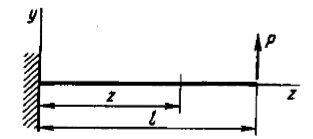
\includegraphics[width=0.5\textwidth]{pic.7}%
	\caption{Балка в заделке}
	\vspace*{-2mm}
	\label{pic7}
\end{figure}

\subsubsection{Метод начальных коэффициентов}
Рассмотрим граничное условие:
\begin{equation}
	\label{graneq11}
	y = 0;\mbox{ } \theta = 0\mbox{, при } z = 0.
\end{equation}

Распределенная сила $q_{y}$ равна  0, так как она не приложена. Найдем момент $M$:
\begin{equation}
	\label{z111}
	\frac{d M}{d z} = P \Rightarrow M = \int\limits_z^l P d z = P(l - z).
\end{equation} 
Далее ищем угол наклона сечения $\theta$:
 \begin{equation}
 	\label{z112}
 	\theta = \frac{P}{E J_{x}} \int\limits_z^l (l - z)d z = \frac{P}{E J_{x}} (\frac{z^2}{2} - l z + c_1).
 \end{equation} 
Получаем уравнение изгиба балки: 
 \begin{equation}
	\label{z112}
	y = \frac{P}{E J_{x}} \int\limits_z^l (\frac{z^2}{2} - l z + c_1) d z = \frac{P}{E J_{x}} (\frac{z^3}{6} - \frac{z^2 l}{2} + c_1 z + c_2).
\end{equation}
Найдем $c_1$ и $c_2$. Для этого рассмотрим граничные условия~(\ref{graneq11}), из них следует, что $c_1 = 0$, поскольку $y(0) = 0$, а $c_2 = 0$, так как $\theta(0) = 0$. Получим итоговое уравнение: 
\begin{equation}
	\label{z1diff}
	y = \frac{P}{E J_{x}} (\frac{z^3}{6} - \frac{z^2 l}{2}).
\end{equation}
Максимальны прогиб будет равен $y_{max} = \frac{P l z^2}{E J_{x} 2}$ при $z = l$. Уравнение изгиба балки будет иметь следующий график:
\begin{figure}[!h]
	\centering
	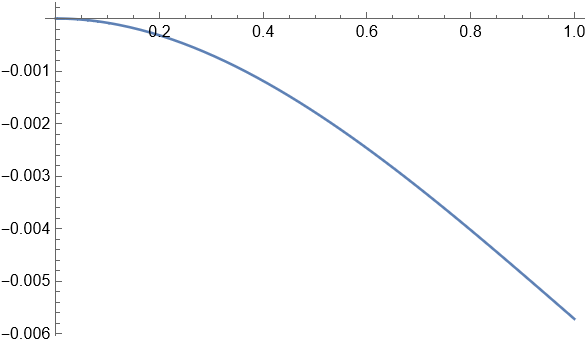
\includegraphics[width=0.5\textwidth]{g.1}%
	\caption{Упругая линия изгиба балки~(\ref{z1diff})}
	\vspace*{-2mm}
	\label{g1}
\end{figure}

\subsubsection{Метод обобщенных коэффициентов}
Рассмотрим граничное условие:
\begin{equation}
	\label{graneq11}
	y = 0;\mbox{ } \theta = 0\mbox{, при } z = 0.
\end{equation}

Рассмотрим уравнения~(\ref{diffb4}) и функцию Дирихле~(\ref{diraca}). Запишем с помощью выражений~(\ref{diffb4}) и~(\ref{diraca}) начальное уравнение:
\begin{equation}
	\label{z123112}
	E J_{x} y^{IV} = P \delta (z).
\end{equation} 
Интегрируем, согласно~(\ref{dirakint}) получаем: 
\begin{equation}
	\label{z12312312}
	E J_{x} y''' = P H (z).
\end{equation}
Интегрируем~(\ref{heaviint}), согласно~(\ref{dirakint}) получаем:
\begin{equation}
	\label{z312312}
	P \int_l^z  H (z) dz = P H (z) (z - l).
\end{equation}
Найдем угол поворота балки в плоскости сечения:
\begin{equation}
	\label{z31231}
	E J_{x} y' = P \int_l^z P H (z) (z - l) dz = P H(z)(\frac{z^2}{2} - l z) + c_1.
\end{equation}
Получаем уравнение гибкого изгиба балки:
\begin{equation}
	\label{z3123}
	y = \frac{P}{E J_{x}} (\frac{z^3}{6} - \frac{z^2 l}{2}) H(z) + c_1 z + c_2.
\end{equation}
Из граничных условий получаем:
\begin{equation}
	\label{z312233}
	c_1 = 0, c_2 = 0.
\end{equation}
Учитывая, что $H(z) = 1 \mbox{, при } z \leqslant l$, получаем итоговое уравнение изгиба балки
 \begin{equation}
	\label{z1ob}
	y = \frac{P}{E J_{x}} (\frac{z^3}{6} - \frac{z^2  l}{2})
\end{equation}

Таким образом, ответ метода обобщенных функций~(\ref{z1ob}) совпал с ответом способа начальных коэффициентов ~(\ref{z1diff}).
\subsection{Двух опорная балка}
Двух опорный стержень длинной $l$ нагружен силой $P$, расположен на расстоянии a от левой опоры~(рис. \ref{pic8}). Составить уравнение упругой линии.  $E_{Al} = 70 \mbox{ ГПа}, J_{x} = \frac{l h^3}{12}, h = 0.01 \mbox{ м}, l = 1 \mbox{ м}$.

\begin{figure}[!h]
	\centering
	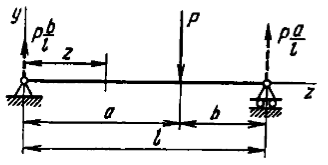
\includegraphics[width=0.42\textwidth]{pic.8}%
	\caption{Двух опорный стержень}
	\vspace*{-2mm}
	\label{pic8}
\end{figure}

\begin{center}Решение\end{center}

\subsubsection{Метод начальных коэффициентов}

Рассмотрим граничные условия:
\begin{equation}
	\label{diffbsec}
	\begin{cases}
		y_1 = 0 \mbox{, при } z = 0\\
		y_2 = 0 \mbox{, при } z = l\\
		y_1 = y_2 \mbox{, при } z = a
	\end{cases}
\end{equation}
Распределенная сила $q_{y}$ равна  0, так как она не приложена. Разобьем стержень на 2 части: до точки приложения $P$ и после. Сила $Q_1 = \frac{P b}{l} $. 
Найдем момент $M_1$:
\begin{equation}
	\label{z221}
	\begin{cases}
		M_1 = \frac{b}{l} \int\limits_0^z P d z = P z + c_0^1 
	\end{cases}
\end{equation}
Параметр $c_0^1 = 0$, так как момент равен нулю (не консоль).
Найдем угол поворота $\theta_1$:
\begin{equation}
	\label{z222}
	\begin{cases}
	\theta_1 = \frac{b}{l} \frac{P}{E J_{x}} \int\limits_0^z P z d z = \frac{b}{l} \frac{P}{E J_{x}} (\frac{b}{l} \frac{z^2}{2} + c_1^1)
	\end{cases}
\end{equation}
Получаем первое уравнение изгиба балки $y_1$: 
\begin{equation}
	\label{z112}
	y_1 = \frac{b}{l} \frac{P}{E J_{x}} \int\limits_0^z (\frac{z^2}{2} + \theta_1) dz =  \frac{b}{l} \frac{P}{E J_{x}} (\frac{z^3}{6} + c_1^1 z + c_2^1),
\end{equation}
Параметр $c_2^1 = 0$, так как концах стержень неподвижен по оси $y$. 

Рассмотрим вторую часть стержня. Сила $Q_2 = \frac{P a}{l}$. 
Найдем момент $M_2$:
\begin{equation}
	\label{z2211}
	\begin{cases}
		M_2 = \frac{a}{l} \int\limits_l^z P d z = -P(z + l)
	\end{cases}
\end{equation}
Найдем угол поворота $\theta_2$:
\begin{equation}
	\label{z2222}
		\theta_2 = - \frac{a}{l} \frac{P}{E J_{x}} \int\limits_l^z P(z + l) d z = - \frac{a}{l} \frac{P}{E J_{x}} (\frac{z^2}{2} + z l - c_1^2). 
\end{equation}
Получаем второе уравнение изгиба балки $y_2$: 
\begin{equation}
	\label{z11332}
	y_2 =  - \frac{a}{l} \frac{P}{E J_{x}} \int\limits_l^z (\frac{z^2}{2} + z l - c_1^2) dz = - \frac{a}{l}  \frac{P}{E J_{x}} (\frac{z^3}{6} + \frac{z^2 l}{2} - c_1^2 z + c_2^2),
\end{equation}
Из граничных условий~(\ref{diffbsec}) получаем:
\begin{equation}
	\label{z113321213}
	c_2^1 = 0,
	c_2^2 = a^3 \frac{1}{6}.
\end{equation}
А так же из граничных условий~(\ref{diffbsec}) получается:
\begin{equation}
	\label{diffbsec2}
	\begin{cases}
		y_1 = y_2\\
		y_1' = y_2'
	\end{cases}
\Leftrightarrow
	\begin{cases}
	{b} (\frac{z^3}{6} + c_1^1 z + c_2^1) = {a}(\frac{z^3}{6} + \frac{z^2 l}{2} - c_1^2 z + c_2^2)\\
	b(\frac{b}{l} \frac{z^2}{2} + c_1^1) = a(\frac{z^2}{2} + z l - c_1^2)
\end{cases}
\end{equation}
Решаем систему ~(\ref{diffbsec2}). Получаем:
\begin{equation}
	\label{z113312213}
	\begin{cases}
		c_1^1 = \frac{a}{6 l} (3 a l - 2 l^2 - a^2)\\
		c_1^2 = -\frac{a}{6 l} (2 l^2 + a^2)
	\end{cases}
\end{equation}
Подставляем в уравнение $y_1$ и $y_2$, получаем:
\begin{equation}
	\label{z2diff}
	y(z) = 
	\begin{cases}
		y_1 = \frac{P}{6 E J_{x}} \frac{b}{l} (z^3 - \frac{2}{3} z l(2 l - \frac{2}{3}l))\mbox{, при } 0 \leqslant z \leqslant a\\
		y_2 = \frac{P}{6 E J_{x}} \frac{a}{l} (-z^3 + 3 z^2 l - z(2 l^2 + \frac{4}{9} l^2) + \frac{4}{9}l^4)\mbox{, при } a \leqslant z \leqslant b
	\end{cases}
\end{equation}
Пусть $a = \frac{2 l}{3}, b = \frac{l}{3}$, тогда уравнение изгиба балки будет иметь следующий график:
\begin{figure}[!h]
	\centering
	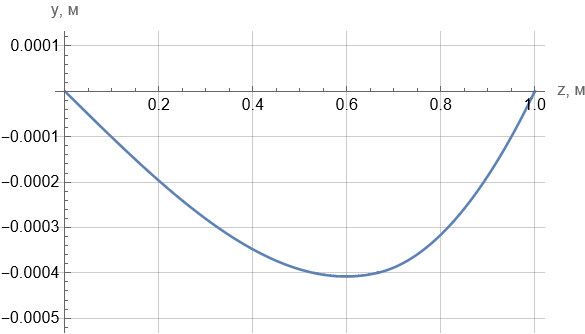
\includegraphics[width=0.5\textwidth]{g.2}%
	\caption{Упругая линия изгиба балки~(\ref{z2diff})}
	\vspace*{-2mm}
	\label{g2}
\end{figure}

\subsubsection{Решение методом обобщенных функций}
Рассмотрим граничные условия:
\begin{equation}
	\label{diffbse12c}
	\begin{cases}
		y = 0, M = 0 \mbox{, при } z = 0\\
		y = 0, M = 0 \mbox{, при } z = l.
	\end{cases}
\end{equation}

Обратимся к источнику~\cite{Birger}.
Рассмотрим уравнения~(\ref{diffb4}) и функцию Дирихле~(\ref{diraca}). 
\begin{equation}
	\label{z1233213}
	E J_{x} y^{IV} = P \delta (z).
\end{equation}
Интегрируем~(\ref{z1233213}), согласно~(\ref{dirakint}) получаем:
\begin{equation}
	\label{z12213}
	E J_{x} y''' = P H (z).
\end{equation}
Найдем момент $M$ согласно~(\ref{heaviint}):
\begin{equation}
	\label{z121334}
	M = P \int_l^z  H (z) dz = P H (z) (z - l).
\end{equation}
Найдем угол поворота балки в плоскости сечения:
\begin{equation}
	\label{z1213}
	E J_{x} y' = P \int_l^z P H (z) (z - l) dz = P H(z)(\frac{z^2}{2} - l z) + c_1.
\end{equation}
Получаем уравнение гибкого изгиба балки:
\begin{equation}
	\label{z123213}
	y = \frac{P}{E J_{x}} (\frac{z^3}{6} - \frac{z^2 l}{2}) H(z) + c_1 z + c_2.
\end{equation}
Из граничных условий~(\ref{diffbse12c}) $c_2 = 0$. Так же найдем $c_1$ из условия $y(l) = 0$~(\ref{diffbse12c}), обозначающий угол поворота сечения
\begin{equation}
	\label{z12321233}
	c_1 = \frac{P l(3 a^2 z^2 - 3 a l z + l^2)}{6 a^3 E J_{x}}
\end{equation}
Кроме того, $H(z) = 1 \mbox{, при } z \leqslant l$. 
Тогда и  итоговое уравнение изгиба балки имеет вид:
\begin{equation}
	\label{z2ob}
	y = \frac{P}{E J_{x}} (-\frac{z^3}{6} \frac{1}{a} + \frac{(z - \frac{l}{a})^3}{6} H(z - \frac{l}{a}) + \frac{l(3 a^2 z^2 - 3 a l z + l^2)}{6 a^3})
\end{equation}

Пусть $a = \frac{2 l}{3}, b = \frac{l}{3}$, тогда уравнение изгиба балки будет иметь следующий график:
\begin{figure}[!h]
	\centering
	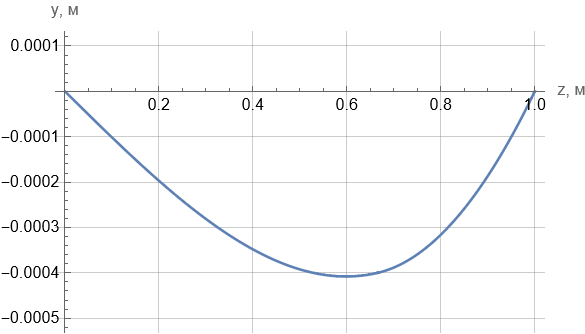
\includegraphics[width=0.5\textwidth]{g.4}%
	\caption{Упругая линия изгиба балки~(\ref{z2ob})}
	\vspace*{-2mm}
	\label{g4}
\end{figure}

Таким образом, график метода обобщенных функций~(\ref{z2ob}) совпал с графиком способа начальных коэффициентов ~(\ref{z2diff}).
\newpage
\section-{Заключение}
В ходе выполнения курсовой были изучены методы начальных коэффициентов и обобщенных функций нахождения уравнения упругого изгиба стержня. Были решены 2 типа задач с помощью этих методов, их результат оказался идентичным. Метод начальных коэффициентов является более трудоемким и менее удобным по сравнению с методом обобщенных функций, поскольку требует учета большего количества граничных условий, больший объем вычислений.
\newpage
\begin{thebibliography}{3}
\bibitem{Feofociev} В.И. Феодосьев Сопротивление материалов: учеб. для вузов. --- 10-е изд., перераб. и доп. --- М.: Изд-во МГТУ им. Н.Э.Баумана, 1999. --- 590 с.	
	
\bibitem{Korneev} Техническая теория стержней. Применение обобщённых функций для решения
задач сопротивления материалов
[Электронный ресурс] : учеб. пособие /
С. А. Корнеев. – Омск : Изд‐во ОмГТУ,
2011.

\bibitem{Birger} И.А. Бригер, Р.Р. Мавлютов Сопротивление материалов: учебное пособие. - М.: Наука Гл. ред. физ.-мат. лит., 1986. --- 560 с.
\end{thebibliography}

\end{document} 